\documentclass[11pt,a4paper]{article}
\usepackage[utf8]{inputenc}
\usepackage[T1]{fontenc}
\usepackage{lmodern}
\usepackage[margin=2.2cm]{geometry}
\usepackage{amsmath}
\usepackage{pgfplots}
\usepackage{pgfplotstable}
\usepackage{booktabs}
\usepackage{tikz}
\usetikzlibrary{arrows.meta,positioning,shapes.geometric}
\usepackage{hyperref}
\usepackage[capitalise]{cleveref}

\pgfplotsset{compat=1.18, width=0.85\linewidth, height=6cm}

\title{Plots and Diagrams}
\author{Your Name}
\date{\today}

\begin{document}
\maketitle

\section{Function plots}
\Cref{fig:functions} is drawn by \texttt{pgfplots} directly from formulas.

\begin{figure}[htbp]
\centering
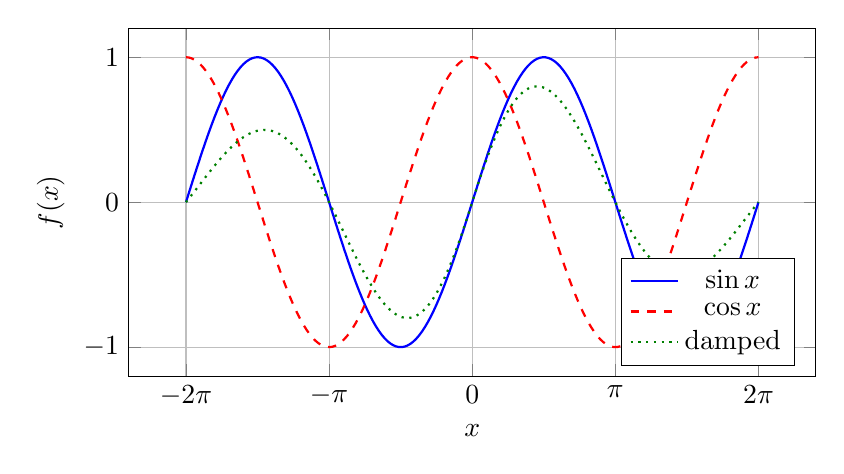
\begin{tikzpicture}
  \begin{axis}[
      xlabel={$x$}, ylabel={$f(x)$},
      domain=-2*pi:2*pi, samples=200,
      legend pos=south east, grid=major,
      xtick={-6.283,-3.1416,0,3.1416,6.283},
      xticklabels={$-2\pi$,$-\pi$,$0$,$\pi$,$2\pi$},
    ]
    \addplot[thick, blue] {sin(deg(x))};
    \addplot[thick, red, dashed] {cos(deg(x))};
    \addplot[thick, green!50!black, dotted] {sin(deg(x))*exp(-0.15*abs(x))};
    \legend{$\sin x$, $\cos x$, damped}
  \end{axis}
\end{tikzpicture}
\caption{Trigonometric functions.}
\label{fig:functions}
\end{figure}

\section{Plotting data from a CSV file}
The measurements in \texttt{data/measurements.csv} are plotted in
\cref{fig:data} and listed in \cref{tab:data}. Edit the CSV file and
recompile to update both.

\begin{figure}[htbp]
\centering
\begin{tikzpicture}
  \begin{axis}[
      xlabel={Time (s)}, ylabel={Value},
      legend pos=north west, grid=both, grid style={line width=.1pt, draw=gray!20},
    ]
    \addplot[mark=*, blue] table[x=time, y=sensorA, col sep=comma] {data/measurements.csv};
    \addplot[mark=square*, orange] table[x=time, y=sensorB, col sep=comma] {data/measurements.csv};
    \legend{Sensor A, Sensor B}
  \end{axis}
\end{tikzpicture}
\caption{Sensor readings loaded from a CSV file.}
\label{fig:data}
\end{figure}

\begin{table}[htbp]
\centering
\caption{The same data as a table, generated by \texttt{pgfplotstable}.}
\label{tab:data}
\pgfplotstabletypeset[
  col sep=comma,
  columns/time/.style={column name={Time (s)}},
  columns/sensorA/.style={column name={Sensor A}, fixed, precision=2},
  columns/sensorB/.style={column name={Sensor B}, fixed, precision=2},
  every head row/.style={before row=\toprule, after row=\midrule},
  every last row/.style={after row=\bottomrule},
]{data/measurements.csv}
\end{table}

\section{Bar chart}
\begin{figure}[htbp]
\centering
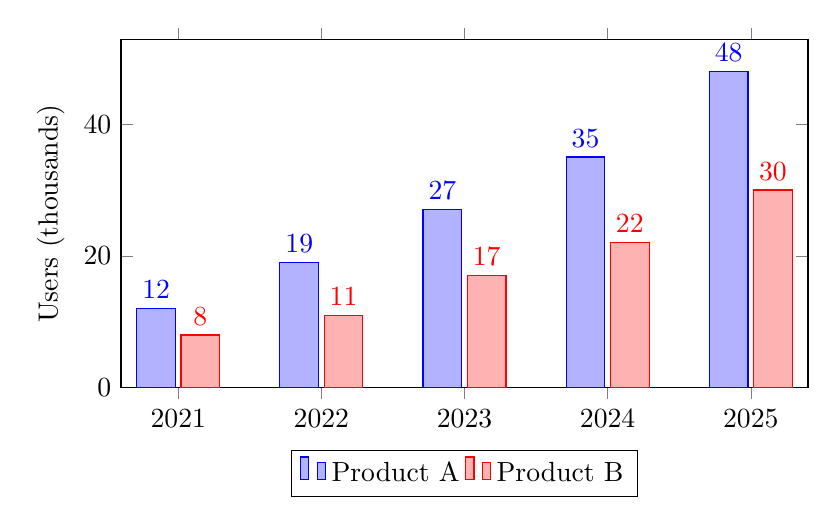
\begin{tikzpicture}
  \begin{axis}[
      ybar, bar width=14pt, ymin=0,
      symbolic x coords={2021,2022,2023,2024,2025},
      xtick=data, nodes near coords,
      ylabel={Users (thousands)},
      legend style={at={(0.5,-0.18)}, anchor=north, legend columns=-1},
    ]
    \addplot coordinates {(2021,12) (2022,19) (2023,27) (2024,35) (2025,48)};
    \addplot coordinates {(2021,8) (2022,11) (2023,17) (2024,22) (2025,30)};
    \legend{Product A, Product B}
  \end{axis}
\end{tikzpicture}
\caption{A grouped bar chart.}
\end{figure}

\section{3D surface}
\begin{figure}[htbp]
\centering
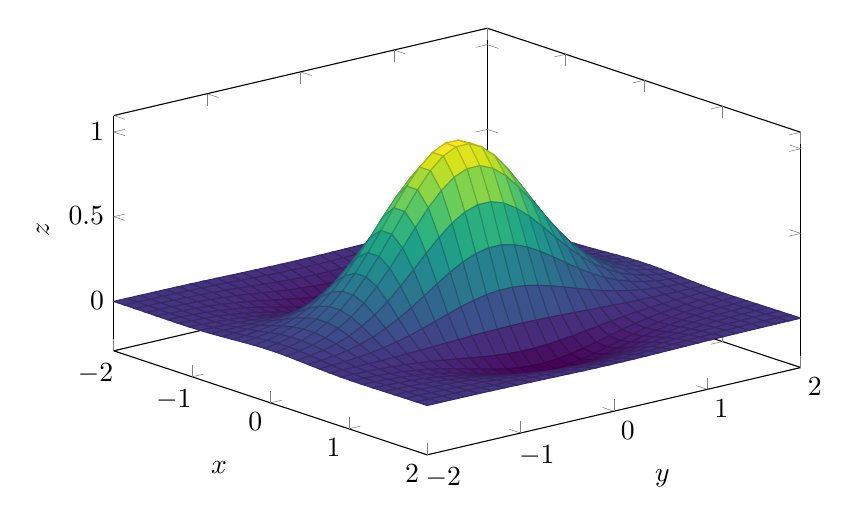
\begin{tikzpicture}
  \begin{axis}[view={50}{30}, colormap/viridis, xlabel=$x$, ylabel=$y$, zlabel=$z$, height=7cm]
    \addplot3[surf, domain=-2:2, samples=30] {exp(-x^2-y^2)*cos(deg(2*x))};
  \end{axis}
\end{tikzpicture}
\caption{A surface plot of $z = e^{-x^2-y^2}\cos 2x$.}
\end{figure}

\section{TikZ diagram}
\begin{figure}[htbp]
\centering
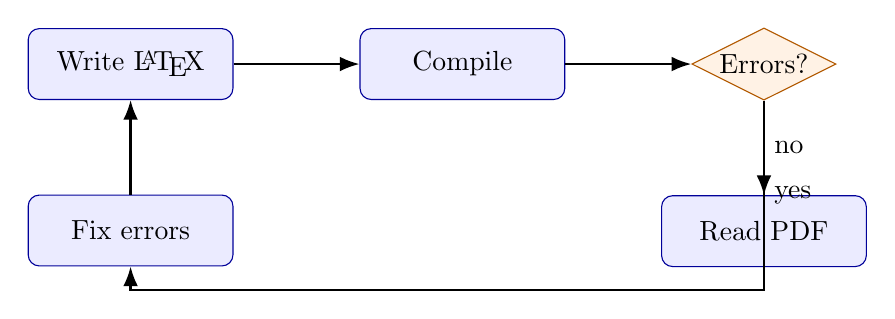
\begin{tikzpicture}[
    node distance=1.2cm and 1.6cm,
    box/.style={rectangle, rounded corners, draw=blue!60!black, fill=blue!8, minimum width=2.6cm, minimum height=0.9cm, align=center},
    dec/.style={diamond, aspect=2, draw=orange!70!black, fill=orange!10, align=center, inner sep=1pt},
    arr/.style={-{Latex[length=2.5mm]}, thick},
  ]
  \node[box] (write) {Write \LaTeX};
  \node[box, right=of write] (compile) {Compile};
  \node[dec, right=of compile] (ok) {Errors?};
  \node[box, below=of ok] (pdf) {Read PDF};
  \node[box, below=of write] (fix) {Fix errors};
  \draw[arr] (write) -- (compile);
  \draw[arr] (compile) -- (ok);
  \draw[arr] (ok) -- node[right] {no} (pdf);
  \draw[arr] (ok) |- node[near start, right] {yes} ([yshift=-2.4cm]ok.south) -| (fix);
  \draw[arr] (fix) -- (write);
\end{tikzpicture}
\caption{A flowchart drawn with TikZ.}
\end{figure}

\end{document}
